\section{Shannon-Weaver Communication Model}
\label{ch1:sec3:overview}

The Shannon-Weaver communication model was first introduced by a paper in 1949 named ``\textit{A Mathematical Theory of Communication}'' by Claude E. Shannon~\cite{shannon1948mathematical}. The main contributions in this paper includes: it first proposed to quantitatively measure the amount of information as \textit{entropy}; it defined communication as ``\textit{\ldots reproducing at one point either exactly or approximately a message selected at another point.}'' This paper established information theory, which had influenced many other disciplines, with applications in data compression, data transmission, speech coding, cryptography, etc. But most of its impact on social sciences only came after Warren Weaver proposed a generalization of the concept communication to encapsulate factors beyond the technical problem, renaming it ``\textit{The Mathematical Theory of Communication}''~\cite{shannon1951mathematical}. With Weaver's interpretation, the communication model now captures the loss of information during the encoding-decoding step. The extended model was widely adopted in areas such as education, communication science, organizational analysis, psychology, etc., which ``\textit{\ldots underlies most aspects of our lives}''. Below we briefly describe the Shannon model and the Weaver model. 

\begin{figure}[h]
\centering
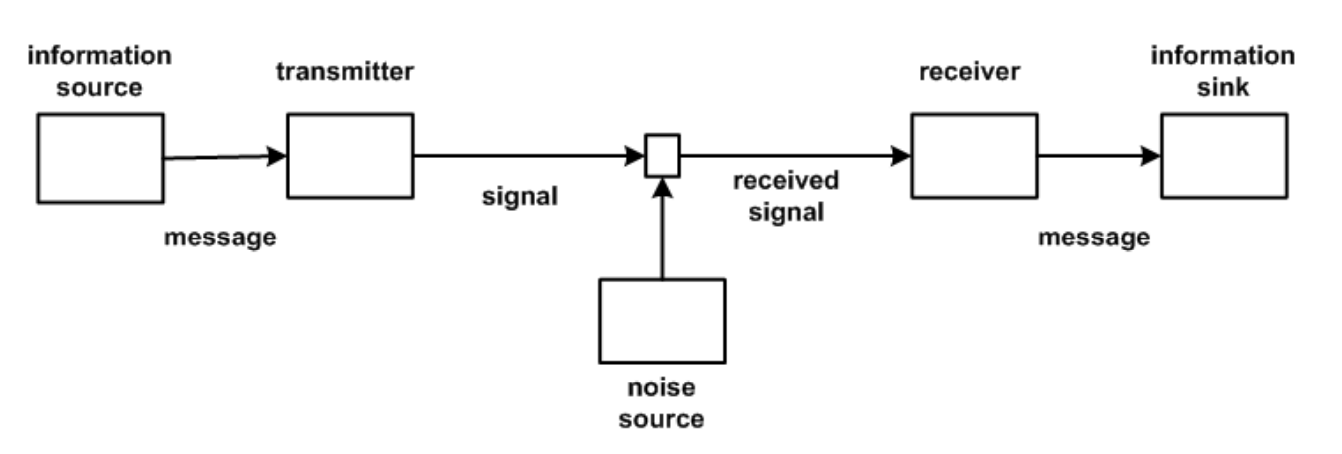
\includegraphics[width=.7\linewidth]{figure/chapter1/shannon}
\caption{Shannon's Communication Model~\cite{shannon1948mathematical}\label{fig:ch1:shannon}}
\end{figure}

\textbf{Shannon's Model}. Shannon's model(Figure~\ref{fig:ch1:shannon}) consists of five components: information source, transmitter, channel, receiver and information sink. The communication starts when an information source is encoded into a message, e.g., it may be encrypted before being transmitted. The encoded message then travels through a transmitter (channel) and reaches the receiver. The channel can be verbal, written, electronic, audio, video, etc. For example, to tell the same story to an audience, one can use either of a video, a voice message or a picture. As the message travels in the channel, the information transmission may be interfered by noise, e.g., a thunderstorm affects the sound signal. Finally, the message is decoded and passed on to the informee. 

\begin{figure}[h]
\centering
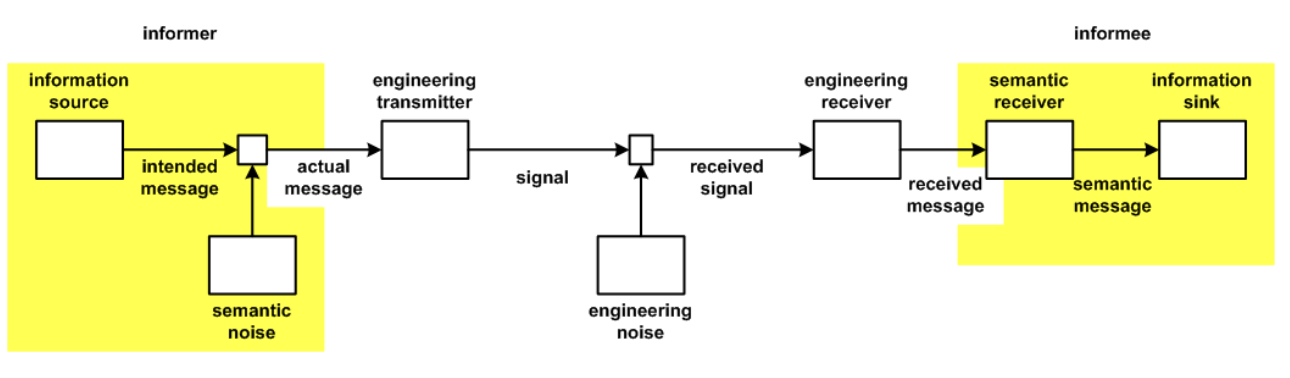
\includegraphics[width=.9\linewidth]{figure/chapter1/weaver}
\caption{Weaver's Communication Model~\cite{shannon1951mathematical}\label{fig:ch1:weaver}}
\end{figure}

\textbf{Weaver's Model}. Shannon's model was developed as a mathematical model for the engineering problem of data transmission. Weaver, however, notice that the communication model can be applied to more general scenarios, e.g., communication where one of the informer and informee is a human. When human is involved, more factors which can influence the communication, e.g., human may produce psychological noise during communication~\cite{miller1967psychology}. Weaver generalized Shannon's model by asking the following questions:

A. (\textit{the technical problem}). How accurately can the symbols of communication be transmitted?

B. (\textit{the semantic problem}). How precisely do the transmitted symbols convey the desired meaning?

C. (\textit{the effectiveness problem}). How effectively does the received meaning affect conduct in the desired way?

While Shannon's model addressed question A, it does not address question B and C. Weaver's model (Figure~\ref{fig:ch1:weaver}) captured two more factors of noise: first, \textit{semantic noise from informer}. when the message was being encoded, the actual message may be different than the intended message due to semantic reasons (instead of technical reasons), e.g., the message sender does not have the full vocabulary to capture the intended meaning. Second, \textit{semantic noise from informee}. When the message was decoded, the semantic message may again differ from the received message. When the informee is a human, the semantically received message relies on what knowledge the informee possess, how much information the informee could process at the same time, etc.~\cite{weavernote}. The two noises may occur by itself or at the same time. A simple example is when a non-native speaker talk to a native speaker, vs. when two non-native speakers (from different countries) talk to each other. 

\textbf{A limitation of Shannon-Weaver Model}. One limitation of Weaver's model is that it fails to capture the context in communication, later work extended the model to address more contextual factors~\cite{chandler1994transmission}. Essentially, the message, informer, informee and channel may all be the same but have different results of deliveries due to different contexts, such as location. The message \textit{let's see a movie tonight} may either refer to watching a movie in theater or at home, depending on whether a theater is available in the location. 

This thesis focuses on studying the semantic noise during the communication process between a mobile system and the mobile user. That is, one of the informee and informer is the human user, the other is a system that communicates with the user through the channel of mobile user interface. In other words, the theoretical framework this thesis is based on is Weaver's model, we do not focus on the engineering noise in Shannon's model. 

\section{System-User Communication in Natural Language}

Natural language interface allows users to communicate with the system in an easily understandable way. Although the term natural language interface typically refers to a system that supports natural language input, here we generalize the concept to also include the discussion on natural language output. 

\subsection{Natural Language Input Interface}

When used as the input, natural language is mainly for \textit{command} (Section~\ref{sec:ch1:why}). The user submits a command in the form of natural language for the system to perform tasks, e.g., web search system, question answering system, speech recognition system, machine translation system, and grammar suggestion systems. Natural language is also used for \textit{satisfy} where the user specifies her requirements in natural language documents. 

Under certain scenarios, the contexts in natural language interface is important for the system to understand user intent, so besides the natural language message, the user also passes the context, e.g., demographic information, device, and location. 

\subsection{Natural Language Output Interface}

When used as the output, natural language is mainly for \textit{explain}, i.e., providing information about the outside world. The majority of system interfaces are built with natural language, but such interfaces can be optimized for better communication with users using the following techniques:

\textit{Summarization}: when the original natural language content is too long, the efficiency of communication can be improved by summarizing the content, e.g., search result snippets. 

\textit{Highlighting}: different choices of highlighting words makes a difference in user attention and the effectiveness of browsing natural language interface~\cite{patel2005systems}.

\textit{Adaptation}: the design of natural language interface should be adapted to better fit the size of the device, for example, web contents are often reduced to fit mobile screen. 

\section{An Overview of the Mobile Systems and User Interfaces}

In this section we give an overview of the mobile systems and user interfaces (channel of communication). Mobile system and mobile devices, in particular smartphon devices, have largely popularized during the last decades. The number of sales in 2018 have been around 1.45 billion, and by the year 2017, more than 31\% people worldwide own a smartphone, which had tripled compared with this number in 2011~\cite{smartphonechart}. Such popularity of smartphones is associated with the rise of Android devices, which has dominated the market (77\% market share in 2018). 

\textbf{Android system and applications}. Android is the open source operating system by Google. The first version of Android was introduced in 2008, the current version is Android 9. Android system is built on top of four layers: the Linux kernel, the library and runtime layer written in C, a Java-compatible application framework, and the application layers. For security, unlike iOS apps which are manually inspected by security vendors, Google has been using the Google Bouncer malware scanner to watch over and scan apps in the Google Play store. Besides, Android security solutions include sandboxing apps, which means that one app does not directly interfere with the operating system or other apps. If an app needs to access certain data (e.g., access to the storage system), it must request the data directly from the user, and the user must directly grant such permission before the app can access the data. The permission system, however, has multiple vulnerabilities, such as stand-alone over-priviledge problem and information leakage, inter-process communication (IPC) collusion, permission re-delegation. 

\textbf{Mobile user interfaces}. Today's mobile user interfaces all adopt a similar design, which is based on direct manipulation, using touching inputs to correspond to real-world actions, such as swiping, tapping, and with a virtual keyboard. For screen sizes, market statistics show that the sizes of the most popular devices are between 5 to 6 inch, which contributes to 90\% of the sales. 

\section{The Challenges of End User Communications Over Mobile Devices}
\label{sec:ch1:challenge}

Considering the unique characteristics of mobile devices, including both the mobile system and interface, there are several challenges for a mobile user to communicate with software on the mobile system. Under the Shannon-Weaver model, we are assuming that one size of the informer-informee is the mobile user while the other side is mobile system, and the these three characteristics would create/amplify the semantic noises from the user's side:

\subsection{Challenge 1: Making Security Decisions}

\begin{figure}[h]
\centering
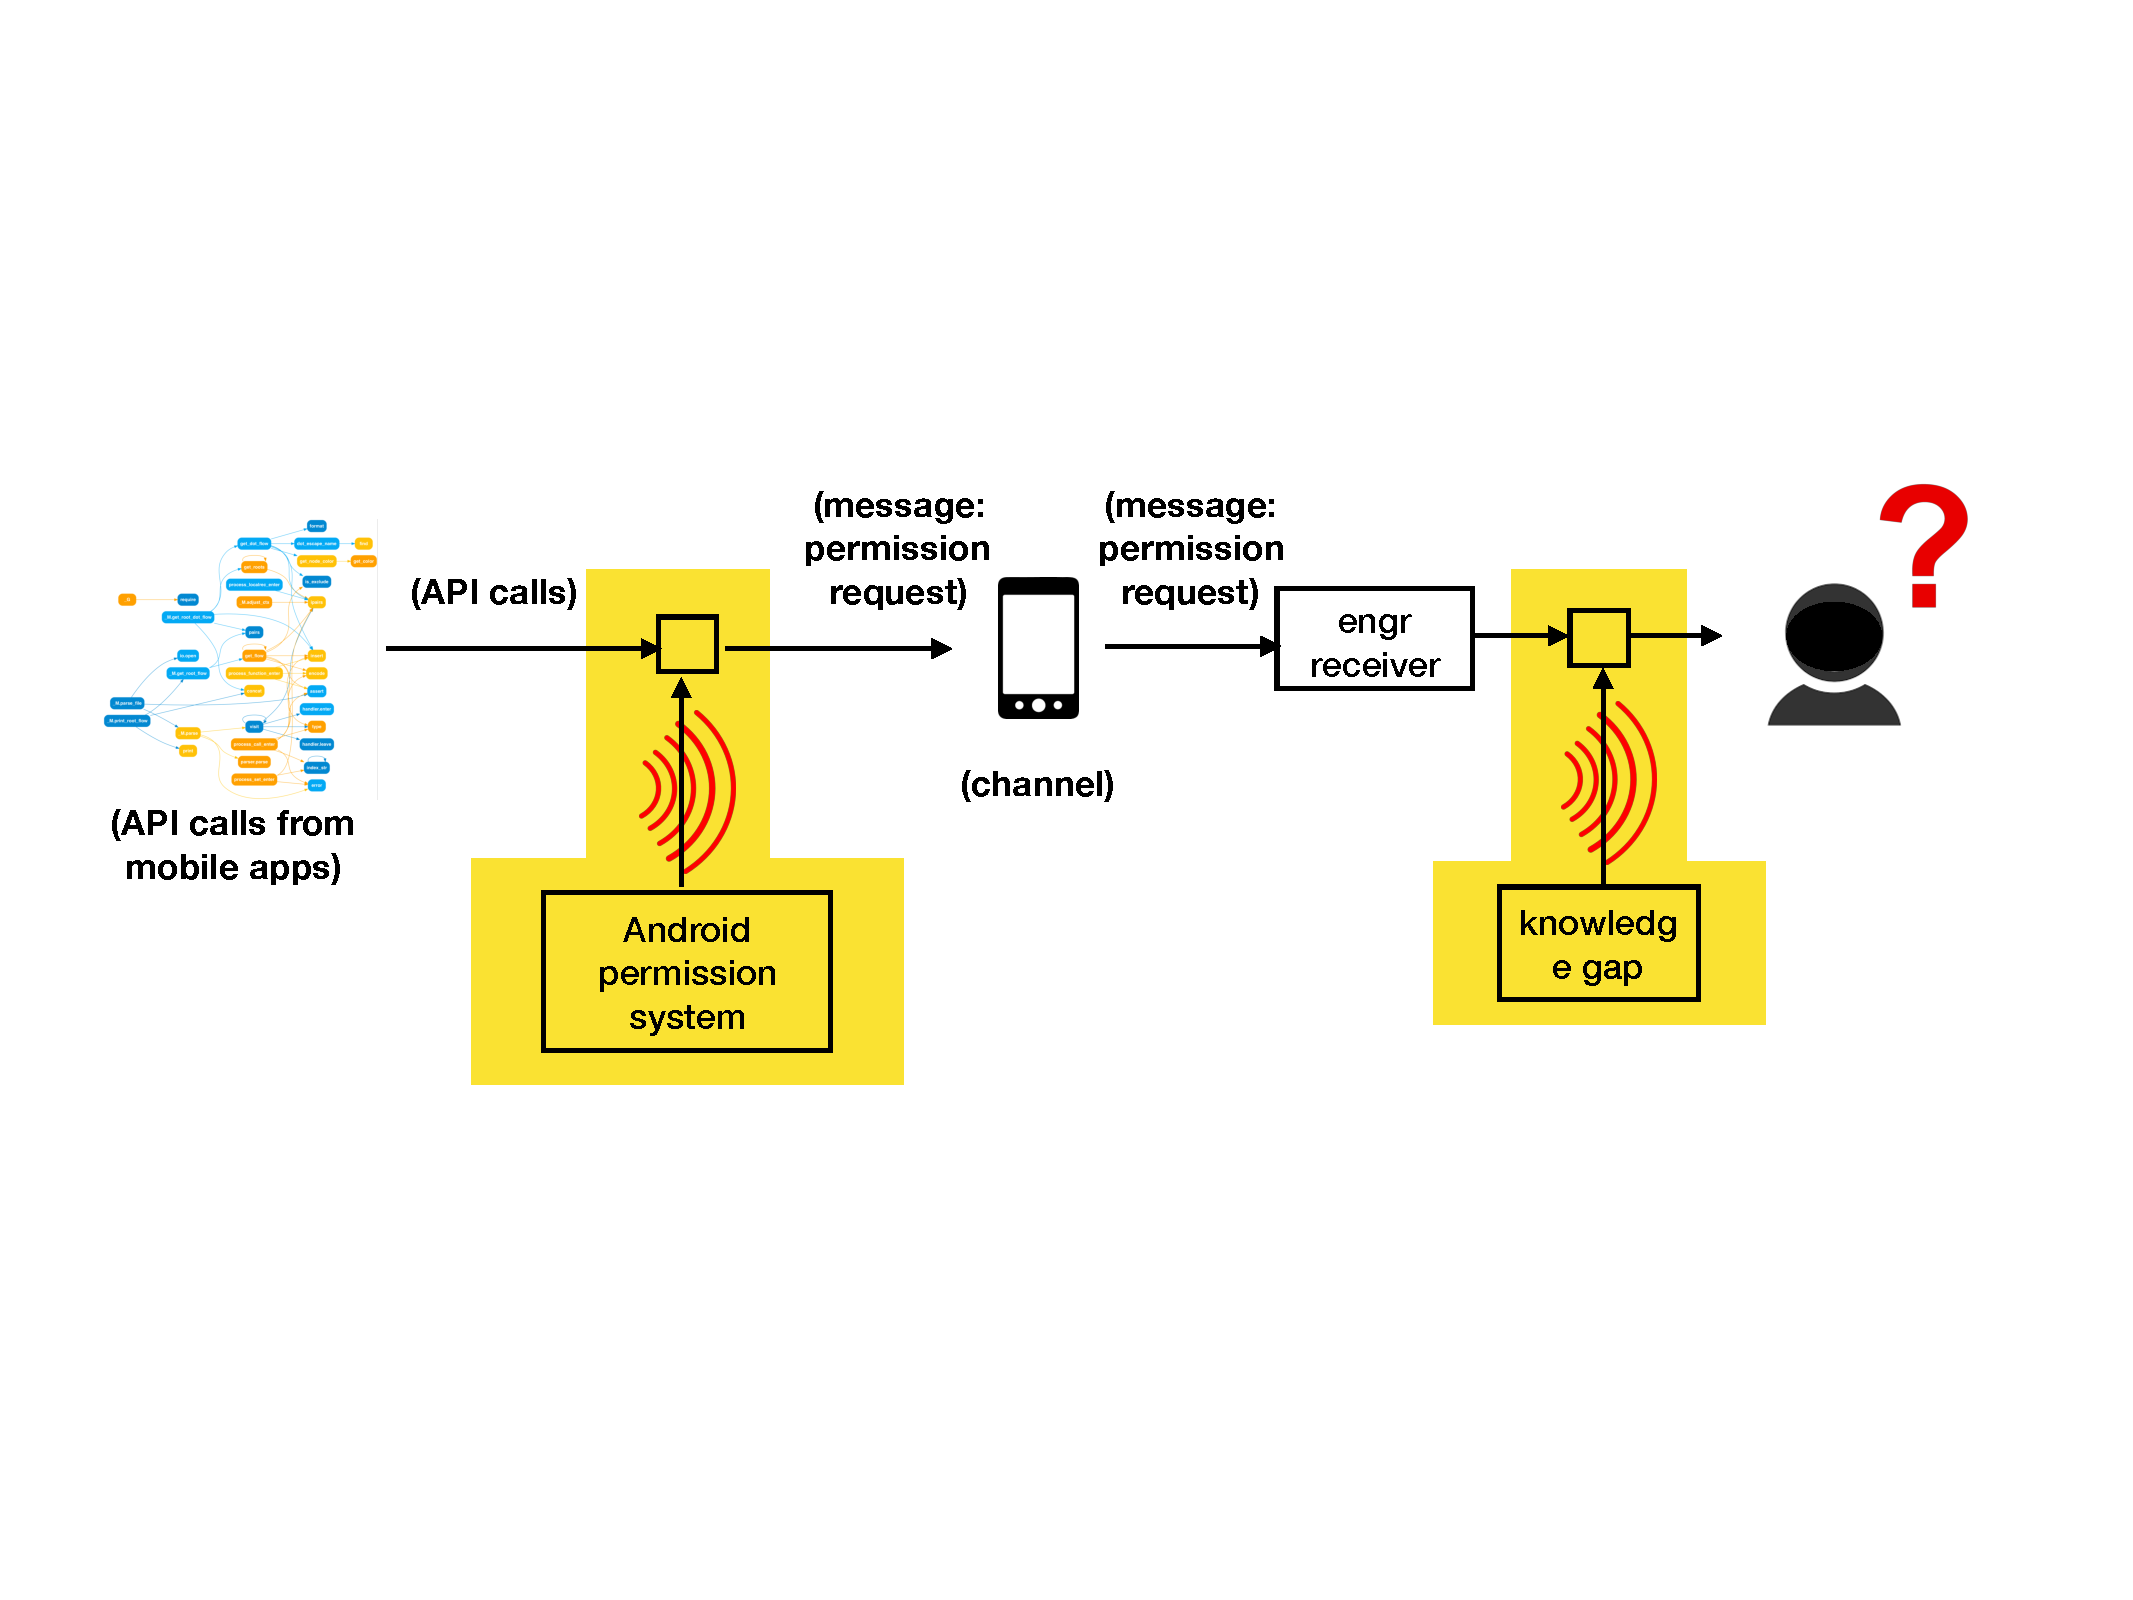
\includegraphics[width=.8\linewidth]{figure/chapter1/system_challenge}
\caption{Due to user knowledge gap and the simplified permission request, the user gets confused on why the app needs permission request\label{fig:ch1:system}}
\end{figure}

One reason for the semantic noise is the knowledge gap between the informer (system) and the user (informee). In a mobile system, often the time the user can just use the app without worrying about how things behind the GUI works, e.g., application layer. However, there exist one case where the user needs to make decisions based on her knowledge about the system, i.e., when user needs to make decision on permission requests. Android relies on users to make decisions on the access to her private information. On the one hand, such design is in accordance to the transparency principle, on the other hand, security depends on the context, e.g., when a GPS app requests the location, such request is legitimate while if a gaming app requests the location, such request may be over-priviledged. There exists too many apps/functionalities than a system-side access control rule could possibly capture, and as a result, the system relies on the user to make the decision. 

To make the permission decision, however, the users need to know why the app needs the permission, and studies show that 1/3 of the time the user cannot understand the reason. In this case, the semantic noise is due to: (1) the message passed contains only the permission request not the purpose of request; (2) the user does not have the knowledge to decode the purpose behind the permission request. 

\subsection{Challenge 2: e-Commerce Shopping}


\begin{figure}[h]
\centering
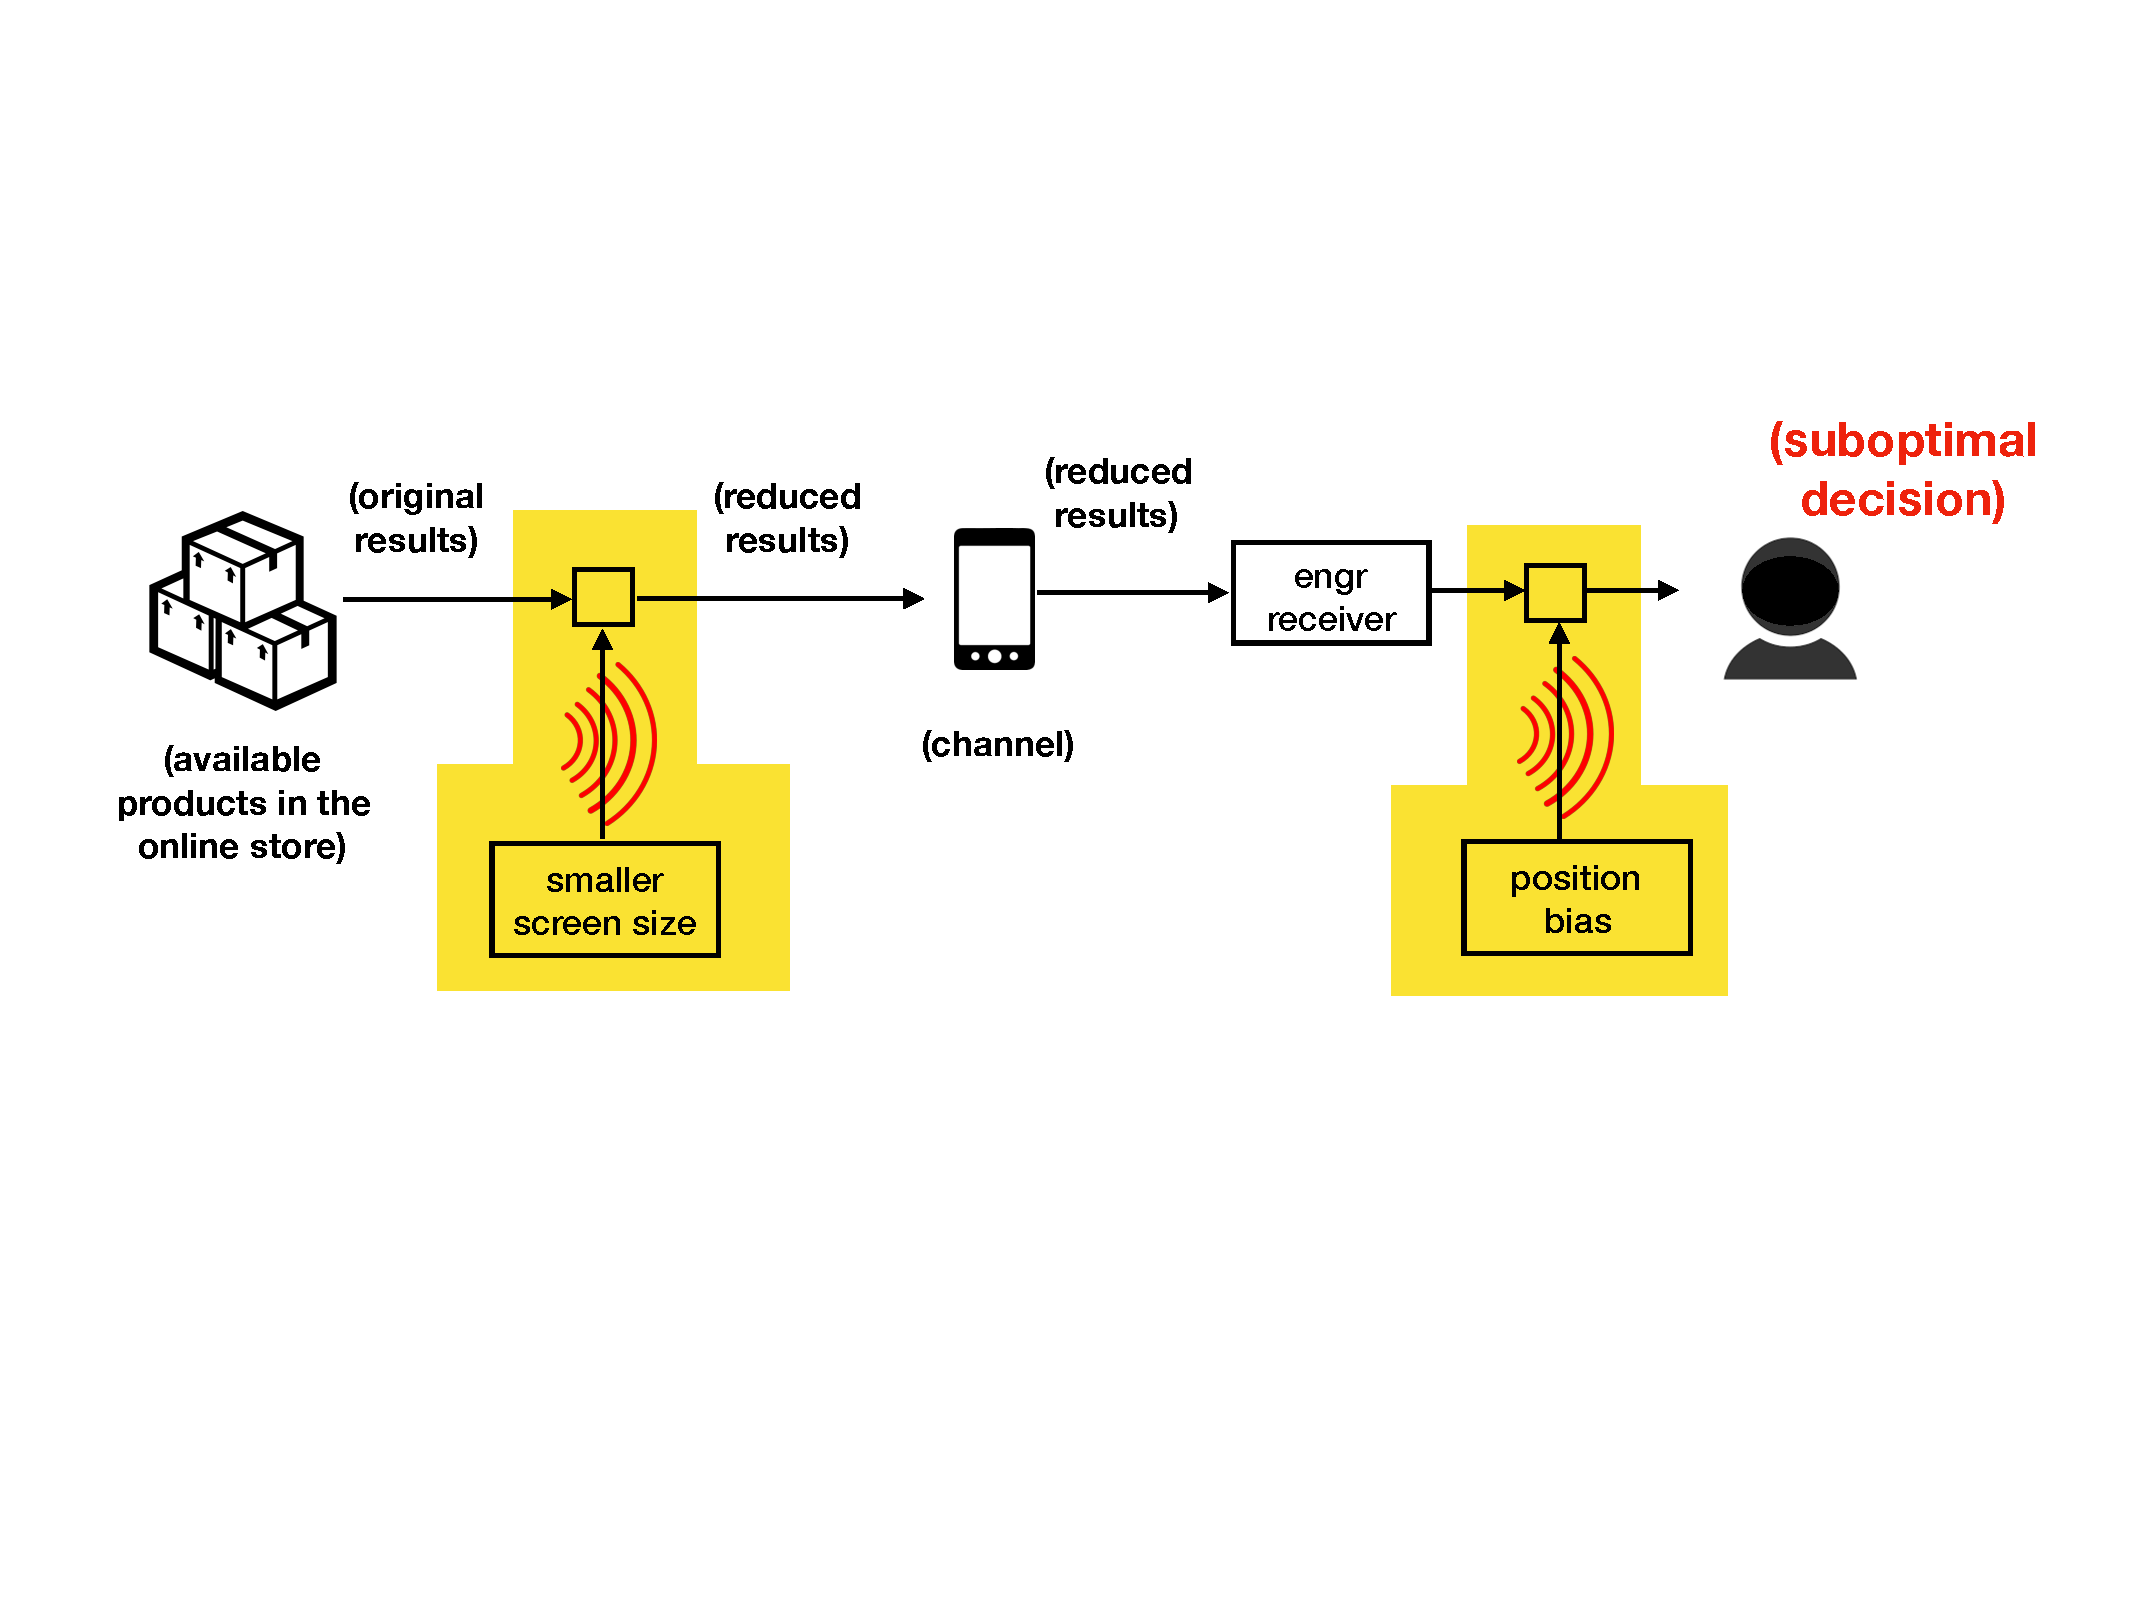
\includegraphics[width=.85\linewidth]{figure/chapter1/gui1_challenge}
\caption{Due to reduced search results and user position bias, the user conduct less exploration of the search results, resulting in the user more likely makes a suboptimal decision\label{fig:ch1:gui1}}
\end{figure} 

\begin{figure}[h]
    \centering
    \subfloat[][Amazon interface on laptop/desktop, which shows the product specification that the mobile interface does not show]{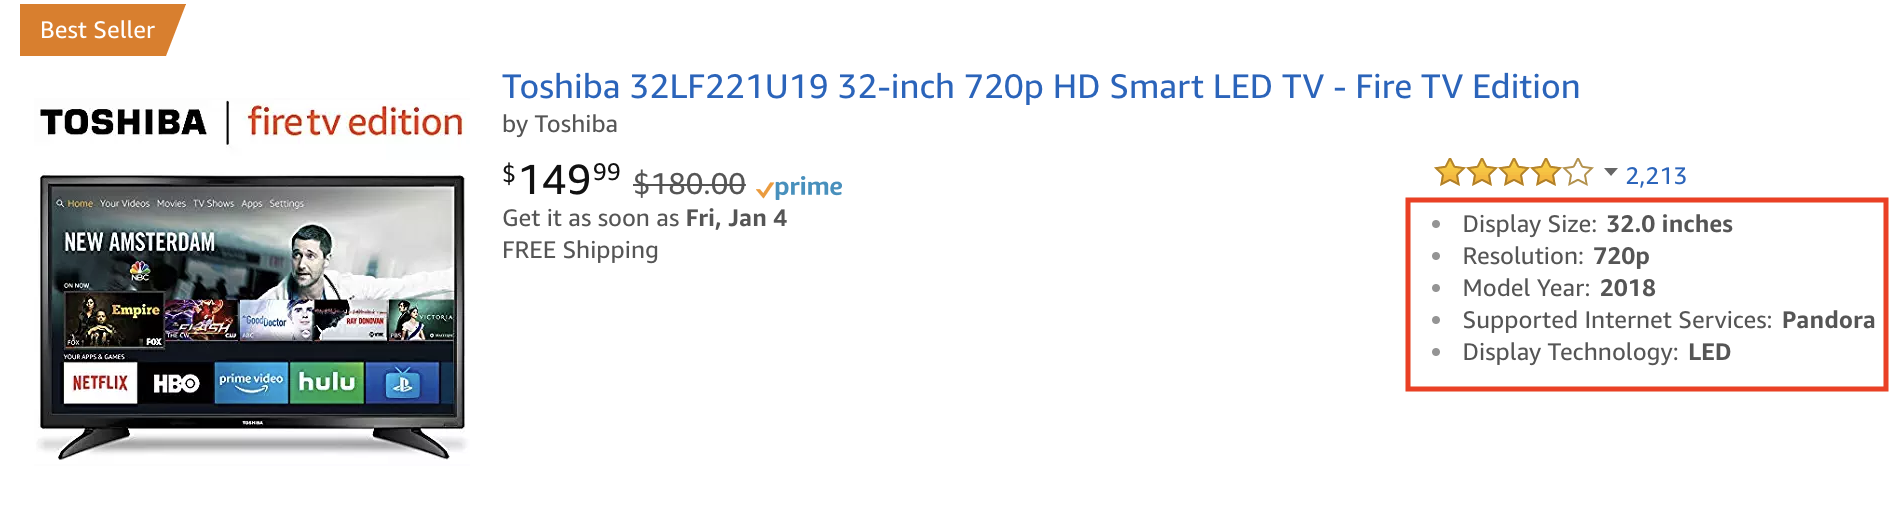
\includegraphics[height=1.2in]{figure/chapter1/amazon_computer}}
    \hfill
    \subfloat[][Amazon interface on phone]{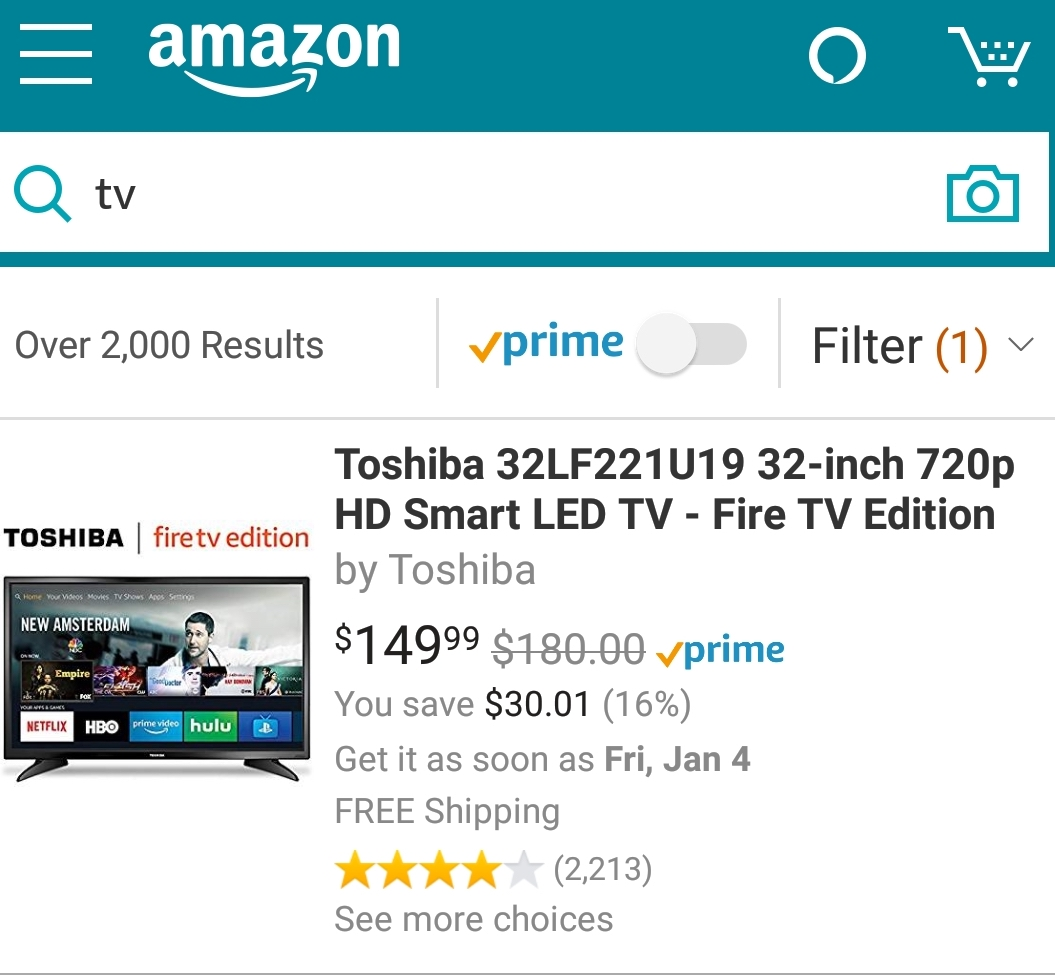
\includegraphics[height=1.2in]{figure/chapter1/amazon_phone}}
    \caption{Difference between display space on laptop/desktop vs. on mobile devices\label{fig:ch1:interface}}
\end{figure}

With the population of mobile devices, more than 40\% e-Commerce purchases are made using a mobile phone~\cite{mobileecom}. However, there exists major challenge for mobile users to explore better options, mostly due to the smaller screen size of mobile devices. As discussed above, most mobile screens are less than 6 inch. The smaller screen gives rise to shrinkage in display space. For example, Figure~\ref{fig:ch1:interface} shows how the interface for the shopping website Amazon is different on mobile devices vs. laptop/desktop devices. With the extra space, the laptop/desktop interface can display the item specification including screen size. The structured specification information are effective in drawing user attention compared with the unstructured item title. 

In the scenario of online shopping, the informer is Amazon and mobile system and the informee is the user customer. The message passed to the channel are all the retrieved produces from Amazon's inventory. However, the customer cannot actually receive all the message, because it would be too time and energy consuming to browse all the products. Among the top ranked products, most users would browse less than 30 items, this phenomenon is called users' \textit{search position bias}, meaning they will pay the most attention to the top ranked items, then the attention decays until the search session is eventually abandoned.

Here the position bias is one type of semantic noise due to two facts: (1) the limited space for display on mobile screens; (2) the cognitive limitation of human users to process information. The effect of position bias is that the user fails to gain a comprehensive understanding on the product specifications before making the decision. The user may think the first product is the best one, before realizing there are TVs with larger screen and the same price in the inventory. 

Notably, users' position bias also exists on laptop/desktop devices, but the bias on mobile devices is much more severe than that on laptop devices. A study by Google in 2017~\cite{ong2017using} finds that users browse 50\% less products on mobile phones, the input less queries in the same search session, and the query words on mobile phones contain less diversified information. All such results indicate users' search on mobile devices lack \textit{exploration}, which means they tend to quickly adopt a sub-optimal result instead of thoroughly exploring more possibilities before making decision. 

\subsection{Challenge 3: Performing Data Analysis}

\begin{figure}[h]
\centering
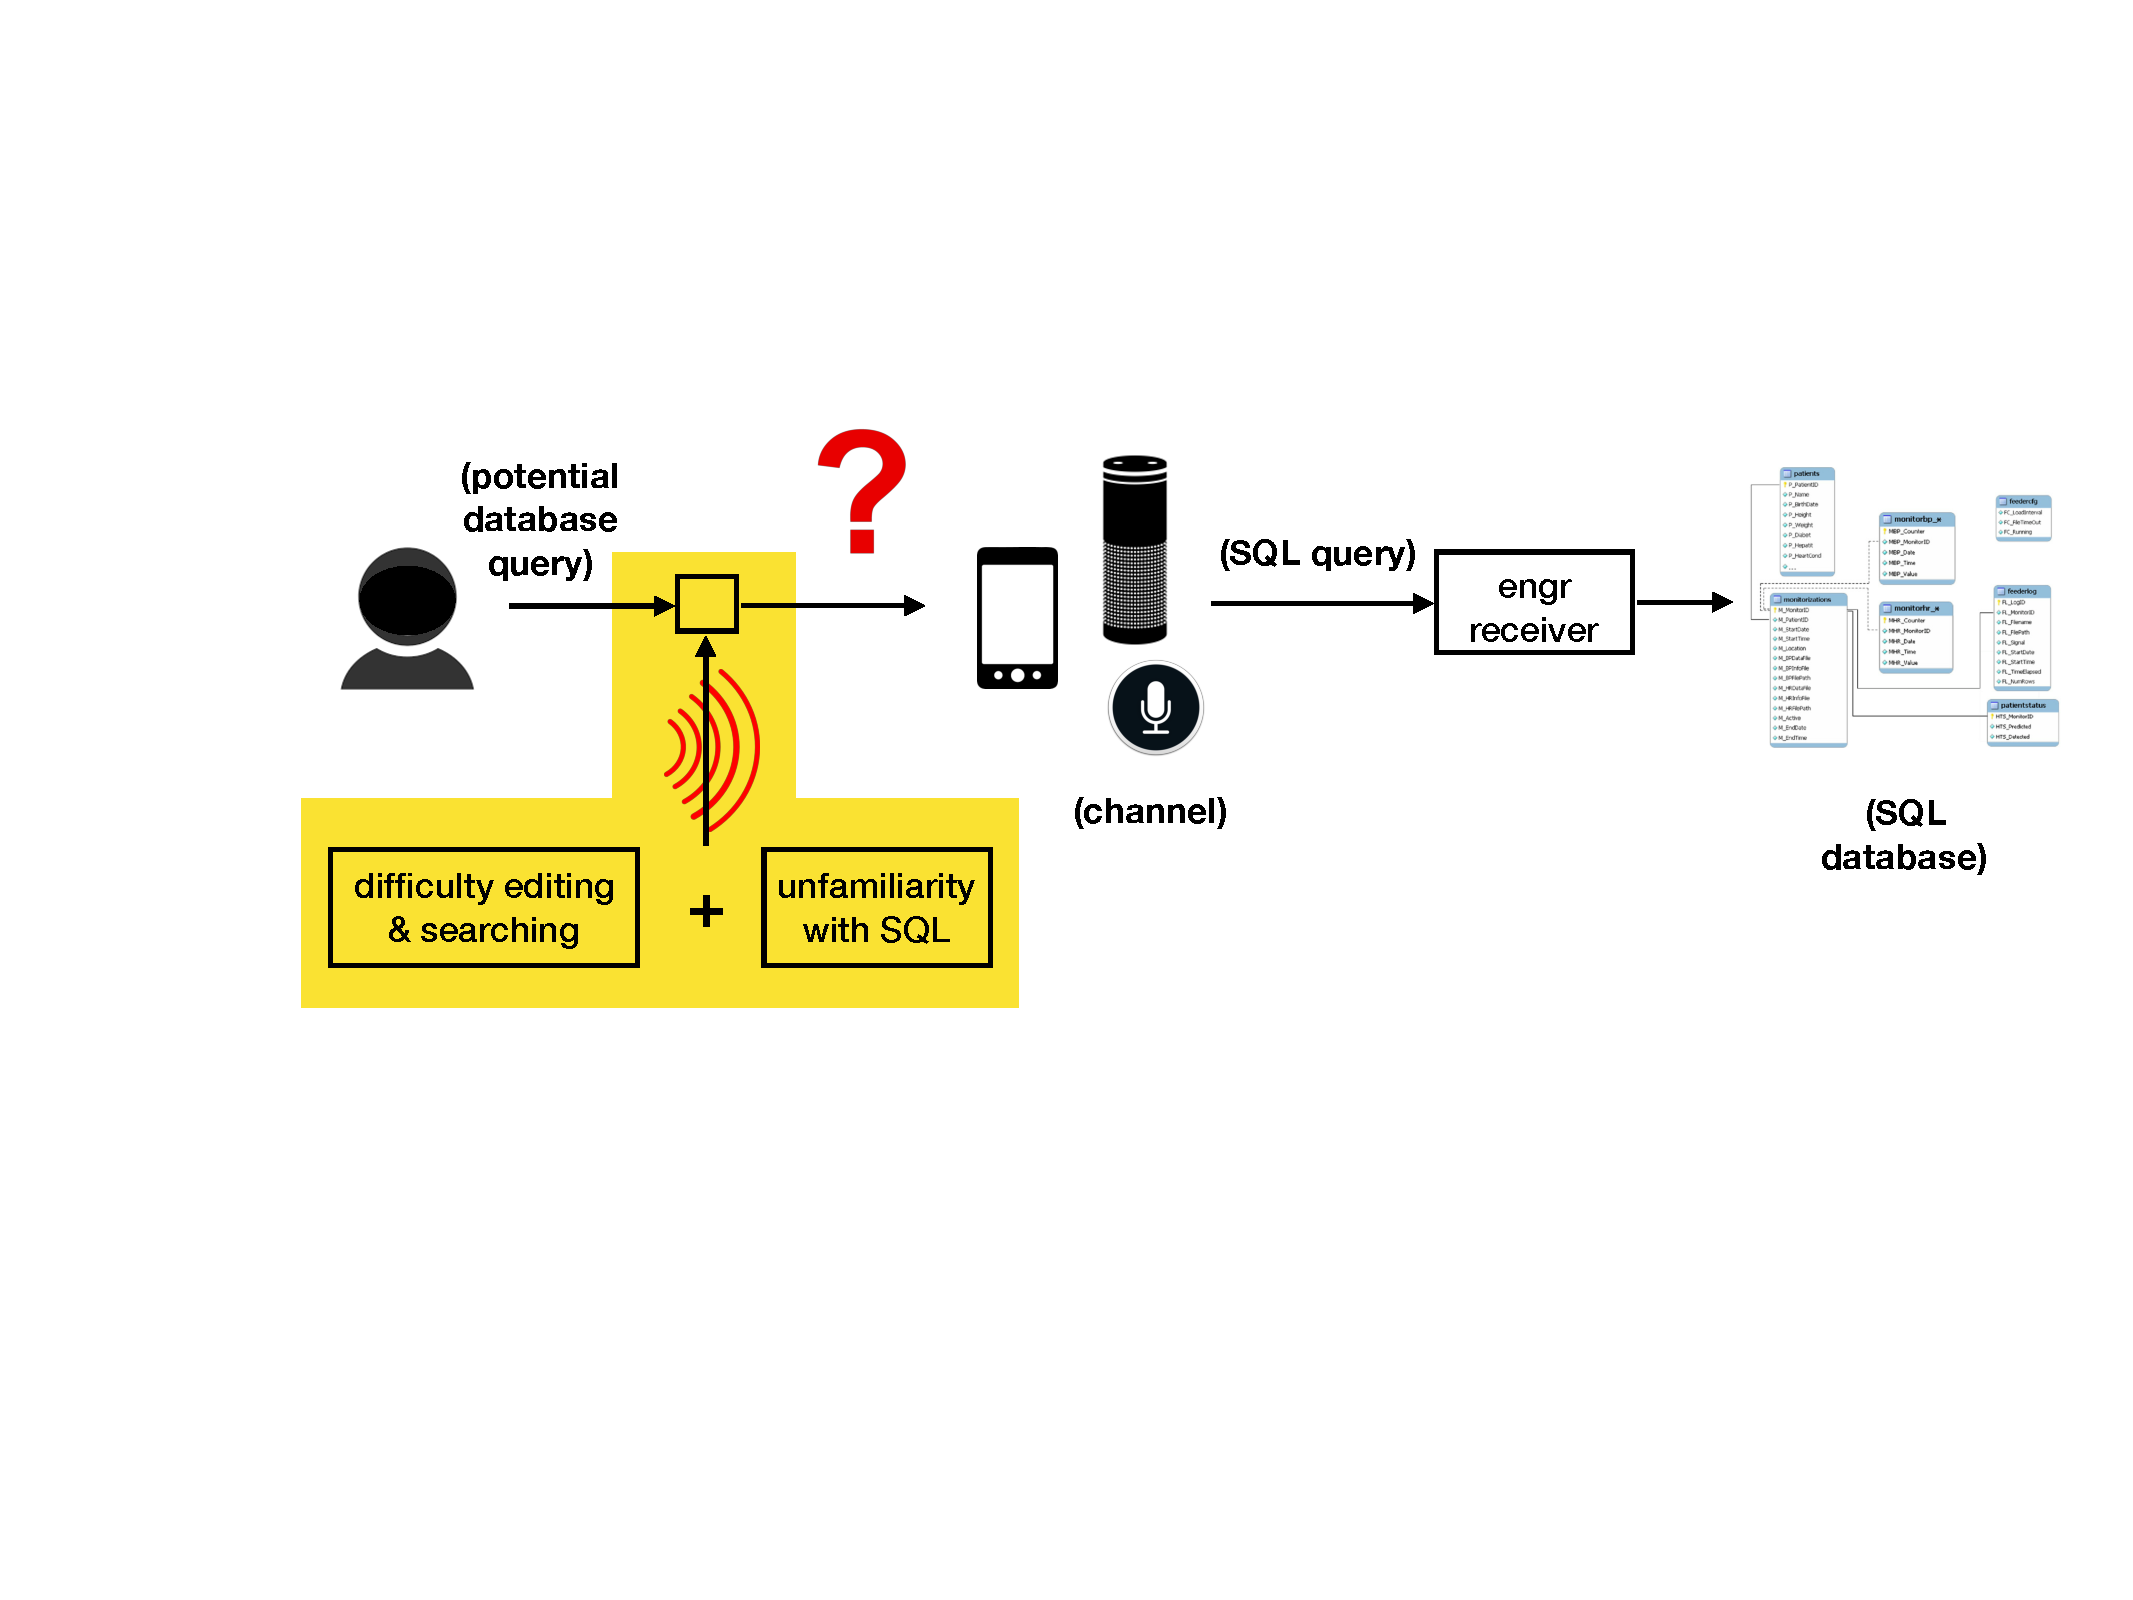
\includegraphics[width=.85\linewidth]{figure/chapter1/gui2_challenge}
\caption{Due to the difficulty to write programs using mobile interface, the user's need to query the database is expressed in natural language, which leads to the disconnection to the database interface.\label{fig:ch1:gui2}}
\end{figure} 

With the population of mobile devices, there is a growing trend of performing data analytics tasks on mobile devices. Companies such as Microsoft, Google, Facebook, Salesforce all launched the mobile app version of their analytics platform, which allows data analytics to perform their tasks on the go. 

Due to the touch inputs on mobile devices, however, it is difficult for data analysts to write database queries for analysis. The touch inputs on mobile phone is slower, more error prone (i.e., fat-finger problem~\cite{siek2005fat}), also requires more attention than on laptops/desktops~\cite{mobiletyping}, This includes the difficulty typing, searching, and copying\&pasting, the latter two are essential operations to support technical inputs. Here the semantic noise comes from: (1) the difficulty for inputing technical information on mobile devices; (2) users' unfamiliarity with database queries (especially beginner analysts). 

\textbf{ Summary on the three challenges}. All the three challenges happens when user's semantic noise meet the nature of mobile devices: small screens, limitations in input efficiency, and a complex and user-dependent security system.